\documentclass{standalone}
\usepackage{tikz}
\usetikzlibrary{mindmap}

\begin{document}
\pagestyle{empty}
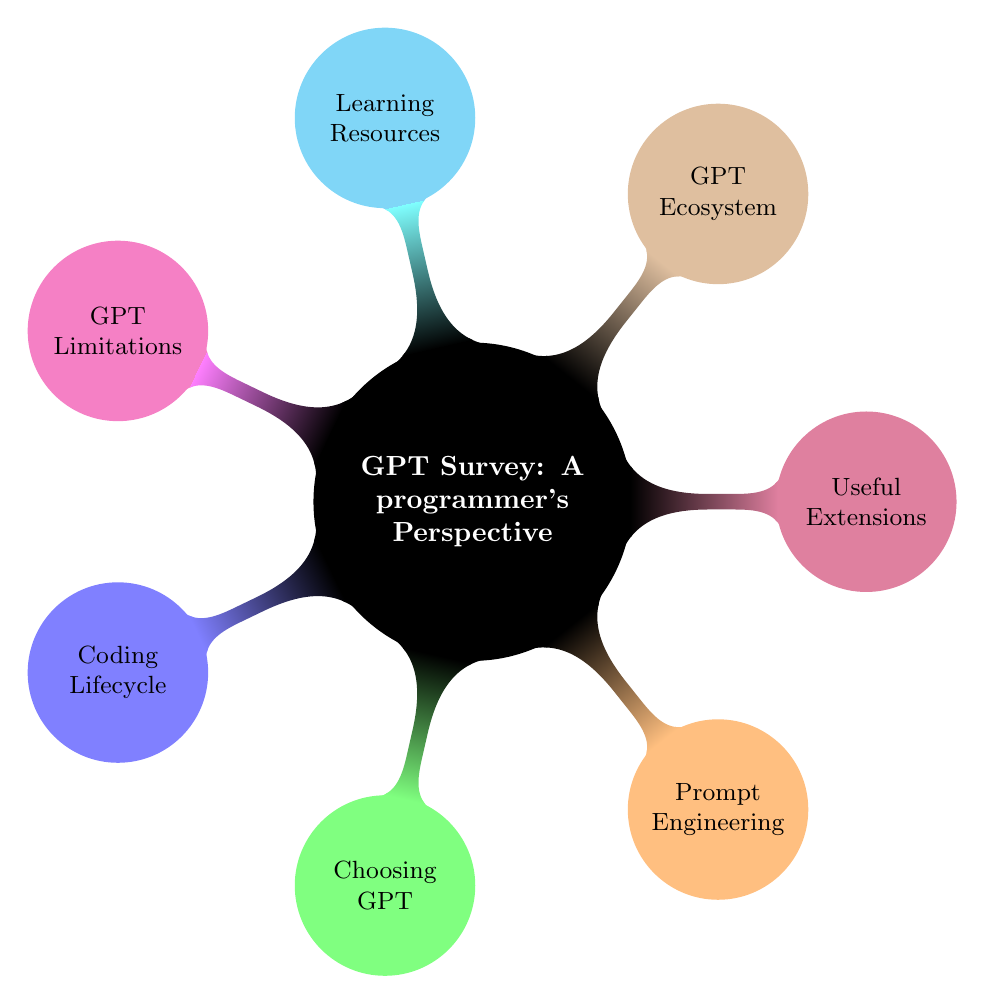
\begin{tikzpicture}[mindmap, grow cyclic,
  every node/.style={concept},
  level 1/.append style={level distance=5cm, sibling angle=360/\the\tikznumberofchildren},
]

  \node[concept color=black, text=white, font=\bfseries] {GPT Survey: A programmer's Perspective}
    child[concept color=blue!50] { node {Coding Lifecycle}}
    child[concept color=green!50] { node {Choosing GPT}}
    child[concept color=orange!50] { node {Prompt Engineering}}
    child[concept color=purple!50] {node {Useful Extensions}}
    child[concept color=brown!50] { node {GPT Ecosystem}}
    child[concept color=cyan!50] {
        node[concept] (n) {Learning Resources}
    }
    child[concept color=magenta!50] {
        node[concept](o){GPT Limitations}
    };
\end{tikzpicture}
\end{document}